\pgfdeclarelayer{background}
\pgfsetlayers{background,main}

\def\sourcesink{{(2, 2)/s}, {(4, 2)/t}}
\def\network{{(2.6, 2.2)/a}, {(3, 1.5)/b}, {(2.25, 1)/c}, {(1.5, 0.8)/d}, {(1, 0.8)/e}, {(2.3, 3)/f}, {(2.7, 3.5)/g}, {(3.3, 3 )/h}}
\def\connect{s/a, a/b, b/c, c/d, d/e, s/f, f/g, g/h, h/t}
\def\connectPath{s-/f, f/g, g/h, h/t-}

\tikzstyle{invis-vertex}=[circle,fill=white!100,minimum size=0pt, inner sep=0pt]
\tikzstyle{vertex}=[circle,fill=black!25,minimum size=10pt,inner sep=0pt]
\tikzstyle{edge} = [draw,thick,-]
\tikzstyle{weight} = [font=\small]
\tikzstyle{real edge} = [draw, line width=8pt,-, gray!70]

\tikzstyle{selected edge} = [draw,line width=5pt,-,gray!50]
\tikzstyle{ignored edge} = [draw,line width=5pt,-,black!20]

\colorlet{circle edge}{black!50}
\tikzset{
  outline/.style={draw=circle edge, thick}
  }

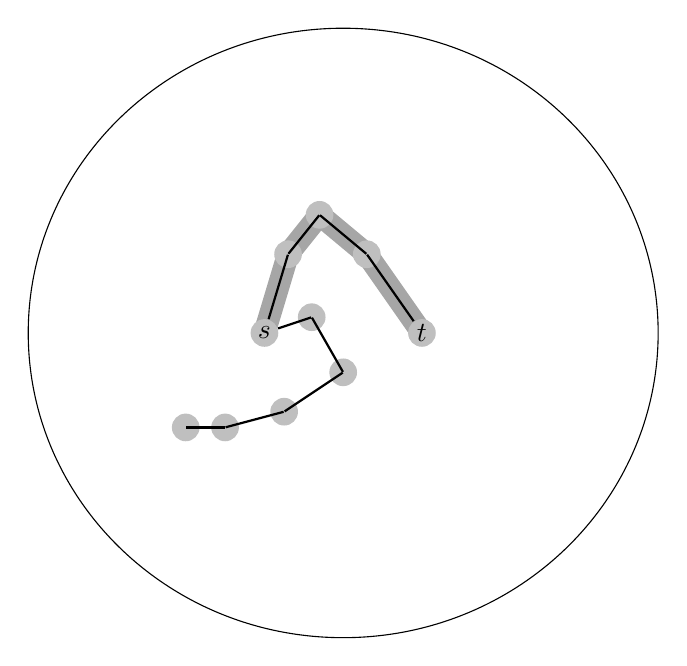
\begin{tikzpicture}
  % First we draw the vertices
  \foreach \pos/\name in \network {
    \node[invis-vertex] (\name) at \pos {};
    \node[vertex] () at \pos {};
  }

  \foreach \pos/\name in \sourcesink {
    \node[invis-vertex] (\name-) at \pos {};
    \node[vertex] (\name) at \pos {$\name$};
  }

  % Connect vertices with edges and draw weights
  \foreach \source/ \dest in \connect
    \path[edge] (\source) -- (\dest);

  \begin{pgfonlayer}{background}
    \foreach \source/\sink in \connectPath
    \path[real edge] (\source) -- (\sink);
  \end{pgfonlayer}        

  \draw (3, 2) ellipse (4 and 3.87);
\end{tikzpicture}
